\subsubsection{การวิเคราะห์การเดินของมนุษย์}
\hspace*{10mm} การเคลื่อนที่ของหุ่นยนต์ฮิวมานอยด์นั้นจะเลียนแบบมาจากการเดินของมนุษย์
ดั้งนั้นการวิเคราะห์ลักษณะการเดินของมนุษย์ จะเป็นการศึกษาเพื่อทำความเข้าใจถึงธรรมชาติการเดิน
ก่อนนำไปทำการออกแบบกลไกทางกลและระบบควบคุมของหุ่นยนต์ฮิวมานอยด์
การก้าวเดินของมนุษย์โดยปกติแล้ว จะมีลักษณะเป็นวัฏจักร วนซ้ำไปเรื่อยๆ ในทิศทางที่ต้องการจนกว่าจะทำการหยุดเดิน
การทรงตัวในระหว่างการยืนหรือการเดินนั้น เป็นไปตามสัญชาติญาณซึ่งเกิดจากการรักษาความสมดุลของระดับน้ำในหู\footnote{text}
ส่งสัญญาณผ่านเส้นประสาทไปยังกล้ามเนื้อส่วนต่างๆ ที่ทำหน้าที่ให้เกิดการเคลื่อนที่ \\
\hspace*{10mm} การเคลื่อนที่ของมนุษย์ในการเดินไปข้างหน้าสามารถแบ่งออกเป็นช่วงต่างๆดังนี้
\\
\begin{figure}[htbp]
    \centering
    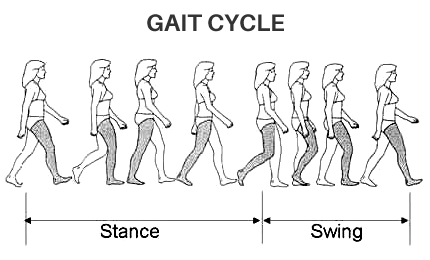
\includegraphics[width=0.55\textwidth]{chapter2/images/gaitcycle.png}
    \caption{วัฏจักรการเดินของมนุษย์}
    \label{fig:human_gait_cycle}
\end{figure}
\begin{enumerate}[label=\arabic*., leftmargin=1.5cm]
    \item ช่วงเริ่มการวางเท้าเพื่อเข้าสู่ช่วงเริ่มต้นเหวี่ยงเท้า เป็นช่วงที่เท้าเกิดการกระแทกลงบนพื้นหลังจากทำการเหวี่ยงมาจากด้านหลัง
    โดยธรรมชาติมนุษย์จะทำการวางส้นเท้าลงเพื่อลดแรงกระแทกที่เกิดขึ้นในช่วงนี้
    ดังนั้นทางกายภาพในส่วนของส้นเท้ามนุษย์จึงมีลักษณะอ่อนนุ่ม
    \item ช่วงเริ่มต้นเหวี่ยงเท้าเพื่อเข้าสู่ช่วงเหวี่ยงเท้า หลังจากทำการวางส้นเท้าลงกับพื้นแล้ว ข้อเข้าจะปรับมุมเพื่อให้ฝ่าเท้าแนบพื้นสนิท
    ขณะเดียวกันขาอีกข้างจะยกสูงขึ้นเพื่อถ่ายเทน้ำหนักไปยังเท้าที่เพิ่งวางลง
	\item ช่วงเหวี่ยงเท้า เป็นช่วงที่ขาหนึ่งยกลอยอยู่ในอากาศและขาที่วางแนบกับพื้นจะรองรับน้ำหนักทั้งหมดของร่างกาย
	\item ช่วงเตรียมการวางเท้า เป็นช่วงที่ขาข้างที่ลอยอยู่เหวี่ยงไปข้างหน้าเพื่อเตรียมเข้าสู่ช่วงรองรับ 
    ในขณะเดียวกันขาที่รับน้ำหนักอยู่จะทำการผลักตัวเพื่อเริ่มทำการถ่ายเทน้ำหนักไปข้างหน้า
\end{enumerate}

\subsubsection{การวิเคราะห์องศาอิสระของมนุษย์}

\subsubsection{กายวิภาคศาสตร์}
